\documentclass[10.5pt]{article}

\usepackage{amsmath}
\usepackage{textcomp}
\usepackage{graphicx}
\usepackage[top=0.8in, bottom=0.8in, left=0.8in, right=0.8in]{geometry}
% Add other packages here %


% Put your group number and names in the author field %
\title{\bf Excercise 4\\ Implementing a centralized agent}
\author{Group \textnumero20 : David Fernandez Navarro, Raphael Madillo}


% N.B.: The report should not be longer than 3 pages %


\begin{document}
\maketitle

\section{Solution Representation}

\subsection{Variables}
We use one unique datastructure called nextTask that contains all usefull variables. This data structure is an HashMap of vehicle with linked list of taskclass. Taskclass is a class that contain a type \{deliver,pickup\} and a task. We use a linked list of taskclass to represent the fact that vehicle will execute each taskclass in order given by linked list.
% Describe the variables used in your solution representation %

\subsection{Constraints}
We have 5 constraints:
\begin{enumerate}
\item The deliver of a task t is always after a the corresponding pickup of t:\\
\[ nextTask.get(v_k).indexOf(tc_i) < nextTask.get(v_k).indexOf(tc_j)\]
\[\textrm{with}\ tc_i.task == tc_j.task \ \textrm{and}\  tc_i.type = pickup \ \textrm{and}\ tc_j.type = deliver\] 
\item A taskclass can be contains by only one vehicle:\\
\[if \ next.Task.get(v_k).contains(tc) \]
\[ then \ \forall v_j \in Vehicle  : \ nextTask.get(v_j).contains(tc) \ is \ false \]
\[ \forall tc \in TaskClass\]
\item If a vehicle carry a taskclass of type pickup and task t then it carry the taskclass of type deliver and task t (and vis-versa):
\[ if \ nextTask.get(v_k).contains(tc_i) \ with \ tc_i.type = \ pickup \ (deliver) \]
\[then \ nextTask.get(v_k).contains(tc_j) \ is \ always \ true \]
\[ with \ tc_j.task = tc_i.task \ and \ tc_j.type = deliver \ (pickup) \]
\item All tasks are pickup and deliver:
\[ \sum_{\forall v_k \in Vehicle} nextTask.get(v_k).size() == 2*TaskSet.size() \]
\item A vehicle is never in overload:
\[ nextTask.getLoad(v_k,time) \leq capacity(v_k) \]
\[with \ time \in \{0 \ ... \ nextTask.get(v_k).size() -1\} \]
\end{enumerate}
% Describe the constraints in your solution representation %

\subsection{Objective function}
% Describe the function that you optimize %
The objective function f can be defined as:
\[f(nextTask) = \sum_{\forall v_k \in Vehicle} \bigg[ \bigg( \sum_{i=1}^{nextTask.get(v_k).size()} tc_{i-1}.getCity().distanceTo(tc_i.getCity) \bigg) + \]
\[ \ v_k.getCurrentCity().distanceTo(nextTask.get(v_k).getFirst()) \bigg]*v_k.costPerKm() \]
And we search for a solution that minimize this cost. 

\section{Stochastic optimization}

\subsection{Initial solution}
As an initial solution we distribute the task randomly on vehicles.
Moreover the pickup and delivery on same task are placed together.
% Describe how you generate the initial solution %

\subsection{Generating neighbours}
We generate neighbours first by changing of vehicle for a task.
We randomly choose a vehicle, and we take its first taskClass (and its corresponding delivery taskclass).
For each other vehicle we create new solutions by putting this taskclass at the beginning on each vehicle.\\
We generate neighbours secondly by changing taskclass order inside the same random vehicle.

% Describe how you generate neighbors %

\subsection{Stochastic optimization algorithm}
In SLS we first create an initiale solution as described above. Then we do as many iteration as specified in argument tCondition.
In each iteration we create a set of neighbours solutions. And then choose the neighbour that minimizes the objective function and with pValue probability we select the old solution or the best neighbour as actual solution.
When we have done all iterations we return the computed plan on actual solution. 
% Describe your stochastic optimization algorithm %


\section{Results}

\subsection{Experiment 1: Model parameters}
% if your model has parameters, perform an experiment and analyze the results for different parameter values %

\subsubsection{Setting}
We run the algorithm with five vehicles, 30 tasks, a pValue=0.4. Then we modify the tCondition (the number of iteration of SLS algorithm) and observe its effect.\\
After that we want to observe the effect of pValue (the probability to take a solution inside neighbors set or the old solution inside localChoice method). We run the algorithm with 3 Vehicles 30 Tasks tCondition = 10000 and modifying the pValue .

% Describe the settings of your experiment: topology, task configuration, number of tasks, number of vehicles, etc. %
% and the parameters you are analyzing %

\subsubsection{Observations}
What we can see here is that by changing the tCondition to a small value,  tCondition = 10, make the cost (which is in mean 52350) depends to much on the initialSolution, which is random, so we are not getting a good approach to the optimal solution ( with tCondition = 10000 costs is in mean 31225). The mean is compute with 6 trials of each configuration. It's also important to consider that less iterations take less time.\\
In second part we observe these results: the overall cost with pValue = 0.1 is in mean (with 6 trials) 27370. The overall cost with pValue = 0.9 is in mean (again 6 trials) 30625. An analyze of this result could be that with high pValue we get stuck on a minimum local cost (because we always return the best neighbor), even doing many iterations it's more difficult to reach the global minimum.

% Describe the experimental results and the conclusions you inferred from these results %

\subsection{Experiment 2: Different configurations}
% Run simulations for different configurations of the environment (i.e. different tasks and number of vehicles) %

\subsubsection{Setting}
% Describe the settings of your experiment: topology, task configuration, number of tasks, number of vehicles, etc. %
We run the centralized algorithm with five tasks and five vehicles initially, then we increment the number of tasks.
The goal of the experiment is to show the effect of task number over distribution on vehicles.\\
We also test the computational time of the algorithm when changing the vehicles. 

\subsubsection{Observations}
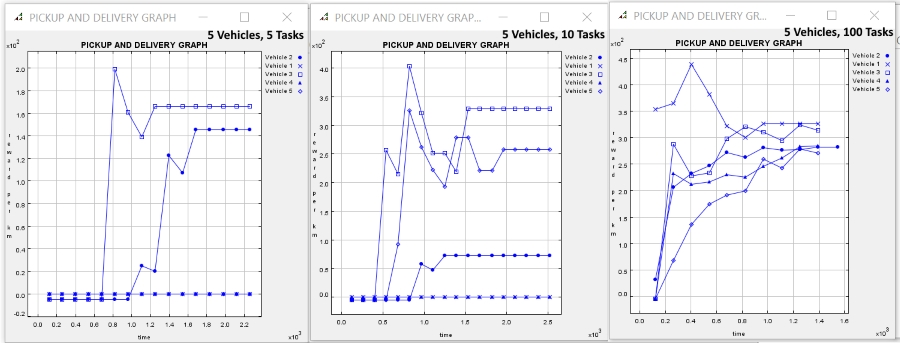
\includegraphics{changinTask.jpg}
\\
With these images we can see the fairness of the algorithm as the number of tasks growth.
When there isn't a lot of tasks we have this result because a vehicle starts its movement it can find another task on its way so it's not worth for the others that remain on their initial cities to move. In contrary when there are many of them, most of vehicles will have a task on their current city so it's now worth pickup and deliver them and also that a vehicle doesn't have enought capacity to take all of them.\\
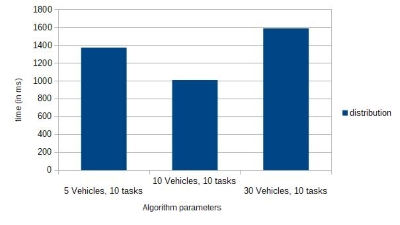
\includegraphics{datagram.jpg}
\\
On this experiment, while seeing the lack of fairness of the algorithm, we also appreciate that for our implementation having less vehicles is not always the best solution when it comes to computation time.
This is because when choosing neighbors, at the swap task function inside a vehicle, if the number of vehicles is smaller for the same amount of tasks, the probability that a vehicle has more tasks is bigger so when we go throw the tasks list of the vehicle, as it’s longer, it takes much more time.
If the number of vehicles is too big we see that time starts incrementing again because of the computation time of the rest of the algorithm.
% Describe the experimental results and the conclusions you inferred from these results %
% Reflect on the fairness of the optimal plans. Observe that optimality requires some vehicles to do more work than others. %
% How does the complexity of your algorithm depend on the number of vehicles and various sizes of the task set? %

\end{document}